\section{Daily markets}\label{sec:market}

\subsection{Data, state and controls}\label{sec:data}

The early-warning state consists of seven trailing-window features of daily S\&P 500 prices and volumes, 3 January 2000 to 16 October 2026: log realized volatility over 20 and 5 days, relative log activity (20-day over 250-day mean volume), the 20-day drawdown and log return, and the rolling 60-day variance of the differenced and lag-one autocorrelation of log 20-day volatility, the standard critical-slowing-down indicators \cite{dakos2012}. Fitted to past data for forecasting, this state is reduced to its first two principal components [PCA(2)]. In the language of Proposition~\ref{prop:decomp} the inputs are the returns $r_t$, their squares and the volume; log volatilities over different windows are filters of one channel, whereas the return and the volatility over the same 20 days are filters of two channels with identical kernels.

Four controls rerun the whole feature pipeline on a modified input (Appendix~\ref{app:surrogates}). Time reversal of the returns and volumes gives $\omega^{\rm rev}$ and, through Eq.~\eqref{eq:estimator}, the two terms. Centered windows remove the observer term (Corollary~\ref{cor:symmetric}). Redrawing the signs of the actual returns removes the coupling between sign and future magnitude and keeps $|r_t|$. Reversible surrogates---an amplitude-adjusted Fourier transform \cite{schreiber1996} of $|r_t|$ with independent signs and phase-matched volume---keep the volatility clustering and are time reversible by construction; a version with symmetric signs removes the drift as well. Bitcoin and Ether states are built in the same way.

\begin{table*}[t]
\squeezetable
\caption{Lag-one antisymmetry of the market states and its decomposition, Eq.~\eqref{eq:estimator}. $\omega$, $\omega^{\rm rev}$ and $\omega^{\rm cen}$ are computed on features from the data, from the time-reversed input and with centered windows; $O=\tfrac12(\omega+\omega^{\rm rev})$, $P=\tfrac12(\omega-\omega^{\rm rev})$. In parentheses, moving-block-bootstrap standard errors in units of the last digit (20-day blocks, 1000 replicates, the three series resampled jointly; 60-day blocks in Table~\Sref{boot}). Surrogates: median [5\%, 95\%] of 200 (S\&P 500) or 100 (Bitcoin, Ether) reversible surrogates. The PCA(2) state is evaluated in the basis of the observed loadings. The centered drawdown is not a symmetric-kernel version of the trailing one (Sec.~\ref{sec:leverage}), so $\omega^{\rm cen}$ does not estimate $P$ in that row.}
\label{tab:markets}
\begin{ruledtabular}
\begin{tabular}{llrrrrrl}
 & channel & $\omega$ & $\omega^{\rm rev}$ & $\omega^{\rm cen}$ & $O$ & $P$ & surrogates\\
\hline
S\&P 500 & window & $-$0.0203(19) & $-$0.0202(21) & $+$0.0013(14) & $-$0.0202(17) & 0.0000(11) & $-$0.023 [$-$0.026, $-$0.020]\\
 & leverage, return & $+$0.0276(34) & $-$0.0276(35) & $+$0.0267(34) & 0.0000(28) & $+$0.0276(21) & 0.000 [$-$0.003, $+$0.004]\\
 & leverage, drawdown & $+$0.0221(30) & $-$0.0108(28) & $-$0.0018(32) & $+$0.0057(22) & $+$0.0165(18) & $+$0.003 [0.000, $+$0.006]\\
 & PCA(2) state & $+$0.0197(32) & $-$0.0206(29) & $+$0.0162(30) & $-$0.0004(25) & $+$0.0202(18) & $+$0.001 [$-$0.003, $+$0.004]\\
\hline
S\&P, to 2020 & window & $-$0.0189(22) & $-$0.0189(23) & $+$0.0004(16) & $-$0.0189(20) & 0.0000(12) & --\\
 & leverage, return & $+$0.0272(37) & $-$0.0263(37) & $+$0.0258(37) & $+$0.0005(28) & $+$0.0268(24) & --\\
 & PCA(2) state & $+$0.0173(29) & $-$0.0174(30) & $+$0.0153(30) & $-$0.0001(22) & $+$0.0174(19) & --\\
\hline
Bitcoin & window & $-$0.0271(28) & $-$0.0289(27) & $+$0.0049(26) & $-$0.0280(22) & $+$0.0009(16) & $-$0.029 [$-$0.033, $-$0.025]\\
 & leverage, return & $+$0.0039(41) & $-$0.0013(42) & $+$0.0041(41) & $+$0.0013(29) & $+$0.0026(30) & 0.000 [$-$0.004, $+$0.004]\\
 & PCA(2) state & $+$0.0049(34) & $+$0.0104(46) & $-$0.0078(40) & $+$0.0076(28) & $-$0.0028(30) & $+$0.007 [$+$0.002, $+$0.012]\\
\hline
Ether & window & $-$0.0309(29) & $-$0.0305(35) & $-$0.0011(33) & $-$0.0307(26) & $-$0.0002(19) & $-$0.036 [$-$0.042, $-$0.032]\\
 & leverage, return & $+$0.0012(36) & $+$0.0012(36) & $-$0.0007(39) & $+$0.0012(24) & 0.0000(27) & $+$0.001 [$-$0.005, $+$0.006]\\
 & PCA(2) state & $+$0.0051(31) & $+$0.0051(43) & $-$0.0095(43) & $+$0.0051(25) & 0.0000(28) & $+$0.006 [$+$0.001, $+$0.012]\\

\end{tabular}
\end{ruledtabular}

\end{table*}

\subsection{The window channel carries the observer term}\label{sec:window}

The volatility windows carry an observer term of the size found in time-reversible surrogates. For log realized volatility over 5 and 20 days the antisymmetry is \OmWinFwd for the data and for the time-reversed input alike, so it is entirely observer term ($|O|$ is \WinOz standard errors), and centering the windows removes it (Table~\ref{tab:markets}). Reversible surrogates, symmetric-sign surrogates and a stochastic-volatility model without leverage give values of the same size [Fig.~\ref{fig:market}(a)]. This is Corollary~\ref{cor:single} in data: the short window leads the long one whatever the direction of time. The OU model fitted to this pair reports $\dot e_p=\,$\EpWinObs per day, and the same model fitted to the surrogates \EpWinSurMed (median)---the large fitted dissipation of the Gaussian observer, now in a market.

\subsection{The leverage channel carries the physical term}\label{sec:leverage}

The physical term is the leverage effect: it reverses under time reversal, survives centering and vanishes when return signs are randomized. For the 20-day return against 20-day log volatility the antisymmetry is \OmLevFwd forward and \OmLevRev backward, so it is entirely physical ($P$ is \LevPz standard errors); it stays at \OmLevCen with centered windows and vanishes in the surrogates [Table~\ref{tab:markets}, Fig.~\ref{fig:market}(b)]. Both features have the same 20-day support, so their observer term vanishes identically (Corollary~\ref{cor:symmetric}); what remains is the odd part of the cross-covariance between returns and later squared returns, the leverage effect \cite{black1976,bouchaud2001} [Fig.~\ref{fig:decomp}(c)]. With linear windows of $r_t$ and $r_t^2$ the decomposition is exact: Proposition~\ref{prop:decomp} evaluated with the empirical cross-covariances reproduces every measured antisymmetry to four decimals in both directions of time (Table~\Sref{prop1}).

The 20-day drawdown, a running maximum and hence a strongly nonlinear filter, shows the limits of the centering control. Equation~\eqref{eq:estimator} attributes most of its antisymmetry with volatility to the physical term ($P=\,$\DDP, $O=\,$\DDO). The centered drawdown, $c_t/\max_{|k|\le10}c_{t+k}-1$, is not a symmetric-kernel version of the trailing one: it responds to losses before $t$ and to gains after $t$ alike, so the two orientations of its lead--lag relation with volatility nearly cancel ($\omega^{\rm cen}=\,$\DDCen). Centering removes the observer term only for features whose centered version is the same functional with a symmetric kernel, whereas time reversal needs no such assumption.

\subsection{What the forecasting state sees}\label{sec:pca}

The forecasting state sees mostly the physical term, because its two leading components discard the direction in which the observer term lives. In the basis of the observed loadings the PCA(2) antisymmetry is \OmPcaFwd forward and \OmPcaRev backward, so the observer term is negligible ($O=\,$\OPcaRev, while $P$ is \PcaPz standard errors); centered windows keep most of it (\OmPcaCen), and the surrogates give zero [Fig.~\ref{fig:market}(c)]. The centering estimate of the observer term, $\omega-\omega^{\rm cen}=\,$\OPcaCen, differs from the time-reversal estimate because the state loads on the drawdown (weights \DDLoadOne and \DDLoadTwo on the two components), whose centered version fails as a control (Sec.~\ref{sec:leverage}). Its fitted entropy production is \EpPca per day, against a median of \EpSurMed, a 95th percentile of \EpSurQ and a maximum of \EpSurMax for the \NSur reversible surrogates (Table~\Sref{surr}): the observed value is \EpObsOverMax times the largest surrogate value. By Proposition~\ref{prop:factor} the excess is a current, not a geometry effect: $\omega_{\rm fit}^2$ is \OmFitSqRatio times and $\mathcal G$ only \GRatio times its surrogate median. The observer term is absent because both volatility features load on the first component with the same sign; their difference, in which the window current lives, falls into a discarded component. Re-fitting the principal components on time-reversed features shows why the size of $\dot e_p$ alone can mislead. The re-fitted plane differs from the observed one, and in it $|\omega_{\rm fit}|=\,$\OmFitRevRefit instead of \OmFitPca while $\mathcal G=\,$\GRevRefit instead of \GPca, so $\dot e_p=\,$\EpRevRefit against \EpPca forward; in the fixed basis of the observed loadings the reversed state has $|\omega_{\rm fit}|=\,$\OmFitRevFixed and $\dot e_p=\,$\EpRevFixed, close to the forward values. By Proposition~\ref{prop:factor} the change lies in the current within a different plane, not in the geometry factor. Every signed comparison is therefore made in one fixed basis.

\begin{figure*}[t]
\centering
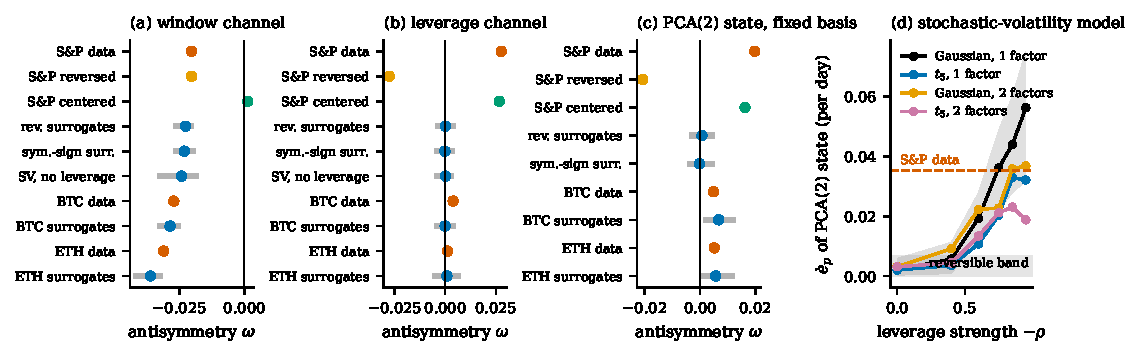
\includegraphics[width=\textwidth]{figures/fig4_markets.pdf}
\caption{In daily markets the volatility windows carry the observer term and the leverage effect carries the physical term. (a) Window channel (log realized volatility over 5 and 20 days): data, time-reversed and centered inputs (colored), reversible and symmetric-sign surrogates, a stochastic-volatility model without leverage, Bitcoin and Ether (median and 5--95\% range for ensembles). (b) Leverage channel (20-day return and 20-day log volatility). (c) PCA(2) forecasting state in the basis of the observed loadings. (d) Entropy production of the PCA(2) state of the stochastic-volatility model against leverage strength for four variants (band: 5--95\% for the Gaussian one-factor model), the S\&P 500 value (dashed) and the reversible-surrogate band (gray).}
\label{fig:market}
\end{figure*}

\subsection{A generative check}\label{sec:sv}

A stochastic-volatility model reproduces the window-channel term and, with leverage, brackets the physical one. Returns are $r_t=e^{h_t/2}\varepsilon_t$ with an autoregressive log variance whose shocks correlate with the previous return shock with coefficient $\rho$ \cite{harvey1996}; the persistence and the coupling of volume to volatility are calibrated to the data, with Gaussian or Student-$t$ shocks and one or two volatility factors (Appendix~\ref{app:data}). Without leverage ($\rho=0$) the median PCA(2) entropy production of every variant lies inside the reversible band and its 95th percentile does not exceed \SVQnfMax, while the full window-channel current is present (Table~\ref{tab:sv}). With leverage strong enough to reproduce the leverage-channel antisymmetry of the data (\OmLevData; medians interpolated in $\rho$), the PCA(2) entropy production is \SVMatchLo--\SVMatchHi per day across variants, bracketing the observed \EpPca [Fig.~\ref{fig:market}(d)]; the Student-$t$ one-factor model reaches at most $\omega_{\rm lev}=\,$\TOneLevMax, where $\dot e_p=\,$\TOneEpAtMax. At $\rho=-0.95$ the Gaussian two-factor model also reproduces the leverage sum $L_+=\sum_{k=1}^{20}\langle r_tr_{t+k}^2\rangle/\langle r_t^2\rangle^2$ of the data. The models bracket the observed values but do not pin them down.

\begin{table}[t]
\caption{Stochastic-volatility null for the PCA(2) state: median entropy production per day, leverage-channel antisymmetry and leverage sum $L_+$ for 30 replicates per leverage coefficient $\rho$, for the simplest and the richest variant (all four in Table~\Sref{sv}).}
\label{tab:sv}
\begin{ruledtabular}
\begin{tabular}{rrrrrrr}
 & \multicolumn{3}{c}{Gaussian, one factor} & \multicolumn{3}{c}{Student-$t$, two factors}\\
$\rho$ & $\dot e_p$ & $\omega_{\rm lev}$ & $L_+$ & $\dot e_p$ & $\omega_{\rm lev}$ & $L_+$\\
\hline
0.00 & 0.0020 & $+$0.0005 & $-$11 & 0.0031 & 0.0000 & 9\\
$-$0.40 & 0.0057 & $+$0.0123 & $-$109 & 0.0044 & $+$0.0139 & $-$176\\
$-$0.60 & 0.0193 & $+$0.0179 & $-$207 & 0.0134 & $+$0.0224 & $-$242\\
$-$0.75 & 0.0362 & $+$0.0243 & $-$222 & 0.0212 & $+$0.0255 & $-$346\\
$-$0.85 & 0.0440 & $+$0.0268 & $-$260 & 0.0231 & $+$0.0287 & $-$337\\
$-$0.95 & 0.0564 & $+$0.0301 & $-$295 & 0.0188 & $+$0.0312 & $-$363\\
\hline
data & 0.0352 & $+$0.0276 & $-$397 & \multicolumn{3}{c}{(same)}\\
\end{tabular}
\end{ruledtabular}

\end{table}

\subsection{Other samples and higher orders}\label{sec:robust}

The split repeats on the 2000--2020 subsample (Table~\ref{tab:markets}). Bitcoin and Ether carry even stronger observer terms in the window channel but no leverage ($|P|\le\,$\CryptoPmax, in the leverage channel less than one standard error); accordingly their PCA(2) states, whose small antisymmetry is mostly observer made, lie inside their reversible bands. Corollary~\ref{cor:single} also marks what second-order window statistics cannot see. The volatility series itself is time asymmetric at third order: the Ramsey--Rothman-type statistic $\sum_{k\le20}\langle z_t^2z_{t+k}-z_tz_{t+k}^2\rangle$ of $z=|r_t|$ is \RRobs, outside the amplitude-adjusted-surrogate range [\RRlo, \RRhi] ($p=\,$\RRp; Table~\Sref{third}) \cite{ramsey1996}. Yet the window channel built from $|r_t|$ is the same forward and backward, as it must be.

\subsection{What the windows cost in information}\label{sec:mktinfo}

The information loss of Sec.~\ref{sec:info} has a market reading. The one-factor stochastic-volatility model calibrated to the autocorrelation of log 20-day volatility (Appendix~\ref{app:data}) relaxes at $\lambda=\,$\LamMkt per day, so the market's 5- and 20-day volatility windows are the first row of Table~\ref{tab:gauss}: even if they averaged the latent log variance itself, they would lose $\ell=\,$\EllMktPair of the information it carries about an excursion beyond $2\sigma$ within ten days, and single windows of 20, 60 and 250 days would lose \EllWinTwenty, \EllWinSixty and \EllWinTwoFifty (Lemma~\ref{lem:mehler}, Table~\Sref{mktinfo}). The pipeline's windows average squared returns instead, a noisy proxy of the variance. In $10^6$-day simulations of the calibrated model the pair of log realized volatilities loses $\ell=\,$\EllMktRV and the PCA(2) state \EllMktPca, estimated as the out-of-sample error of a flexible regression of the oracle on the observation; the same estimator recovers the exact loss of the noise-free pair to within \EllCheckDiff. Most of what the forecasting state does not know about the next volatility excursion is therefore lost to the noise of its inputs rather than to the delay of the windows, and no estimator built on that state can recover it.

